\label{sec:2.2}

%%%%%%%%%%%%%%%%%%%%%%%%%%%%%%%%%%%%%%%%%%%%%%%%%%%
% (GAO) BNL Test System
%%%%%%%%%%%%%%%%%%%%%%%%%%%%%%%%%%%%%%%%%%%%%%%%%%%
 The block diagram of the ColdADC test board at BNL is shown in the Figure~\ref{fig:bnl_testsyst}. There are two types of ColdADC test board at BNL. The first type can have either ColdADC die directly wire-bonded on board or packaged chip populated on the board. The purpose of this board is for ColdADC performance characterization, as shown in Figure~\ref{fig:bnl_testbd1}.  The second type has an ASIC test socket mezzanine on the test motherboard, which is aimed for the QC test, as shown in Figure~\ref{fig:bnl_testbd2}. 
\begin{figure}[!ht]
\centering
 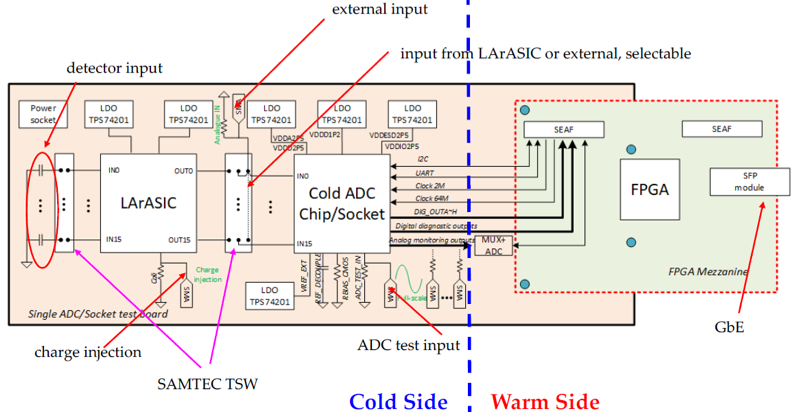
\includegraphics[width=0.85\linewidth]{figures/BNL_testsystem.png}
  \caption{Block diagram of the BNL ColdADC test board}
  \label{fig:bnl_testsyst}
\end{figure}

The test motherboard hosts a P1/P2 LArASIC chip, a ColdADC chip (or die, or ASIC socket mezzanine), a few cold regulators and some passive components (capacitors, resistors and connectors). There are two features different from Fermilab and LBNL test boards. First, this is a test board which can characterize ColdADC performance with the FE-ASIC chip, a full chain from analog detector signal input to digital output is implemented. By using signal generator, we can also characterize standalone ADC performance, including power consumption, INL/DNL, ENOB, DC noise, etc. Second, ColdADC can be powered either by on-board regulators or directly by external power supply, which is not shown in Figure~\ref{fig:bnl_testsyst}. On-board regulators can provide extremely low noise power sources for the test board, which is suitable for noise-sensitive measurements, such as the full chain performance characterization test. Inputs of ColdADC chip can be connected either to FE-ASIC outputs or signal generator outputs.  

To minimize the design effort, a ProtoDUNE FM (FPGA mezzanine board) is adopted to configure LArASIC/ColdADC and read data out.  The FM communicates with computer through Gigabit Ethernet, and UDP protocol is used.
\begin{figure}[!ht]
\centering
 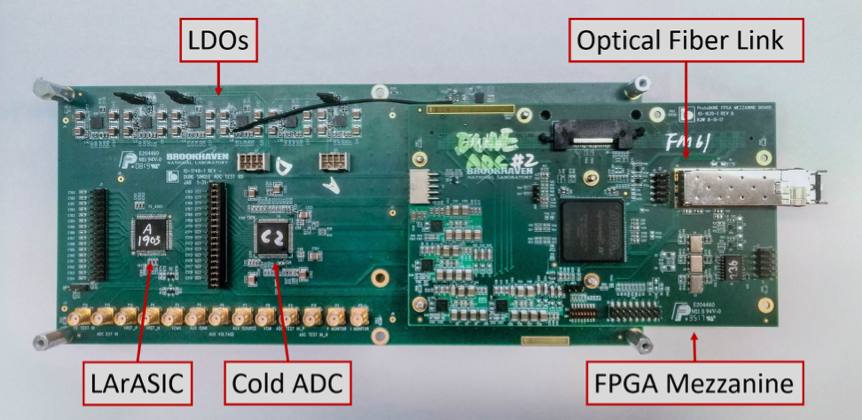
\includegraphics[width=0.85\linewidth]{figures/BNL_testbd1.png}
  \caption{Test board with packaged ColdADC chip. To avoid unexpected noise from computer, a 1-port fiber to copper switch is inserted between FM and the computer.}
  \label{fig:bnl_testbd1}
\end{figure}
\begin{figure}[!ht]
\centering
 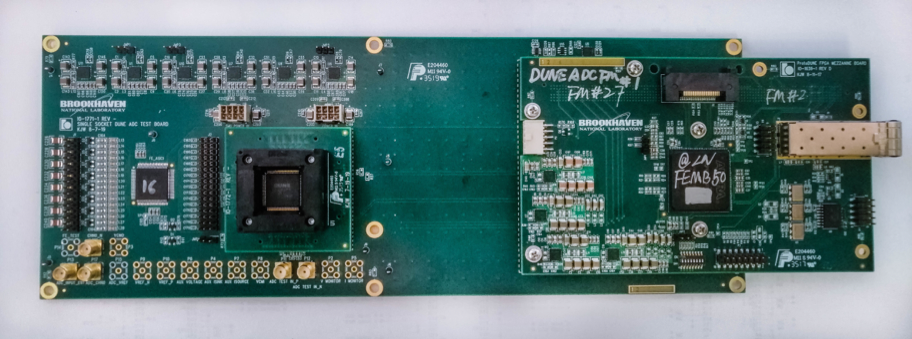
\includegraphics[width=0.85\linewidth]{figures/BNL_testbd2.png}
  \caption{Test board assembly with ColdADC socket mezzanine. The socket test motherboard can be treated as a minor revision of chip/die test motherboard. The socket test motherboard integrates MICA 150pF capacitors at the FE inputs to simulate the capacitance of 8m detector sense wire, which makes the full chain characterization close to the real experiment with the detector.}
  \label{fig:bnl_testbd2}
\end{figure}

As shown in Figure~\ref{fig:bnl_testsetup} is the test setup for ADC performance characterization. Low noise power supply Keysight E36312A is used if ColdADC is powered directly by external power supply. There are 3 different power rails for ColdADC, VDDA2P5/VDDD2P5 is set to 2.5V if CMOS reference is chosen and 2.7V if BJT reference is chosen, VDD1P2 is set to 2.1V, and VDDIO2P5 is set to 2.25V. The power consumption of ColdADC can be measured by power supply. E36312A provides a flexible way to adjust voltages for ColdADC but the noise is not as low as on-board regulators, so for precision measurements, on-board regulators should be used. Power supply Rigol DS832 provides two power rails (5.0V and 2.8V) for both ColdADC test motherboard and FPGA mezzanine. All on-board regulators are powered by DS832. SRS DS360 is an ultra-low distortion function generator with 20-bit resolution and THD lower than -100 dBc, which is sufficient to study ADC INL/DNL and ENOB performance. In addition, we also have a Keysight 33600A generator (14-bit resolution) to provide both ramp and sine waveforms for INL/DNL study if needed (actually in the beginning 33600A was used to characterize INL/DNL with ramp waveform). In order to study ADC dynamic performance such as ENOB, FM outputs 10MHz clock to synchronize SRS360. (Later in the QC test, instead of 100MHz oscillator on board, the CG635 synthesized clock generator is applied to provide a stable 100MHz clock source which is not affected by temperature change, and CG635 outputs a 10MHz clock to synchronize SRS360). 
\begin{figure}[!ht]
\centering
 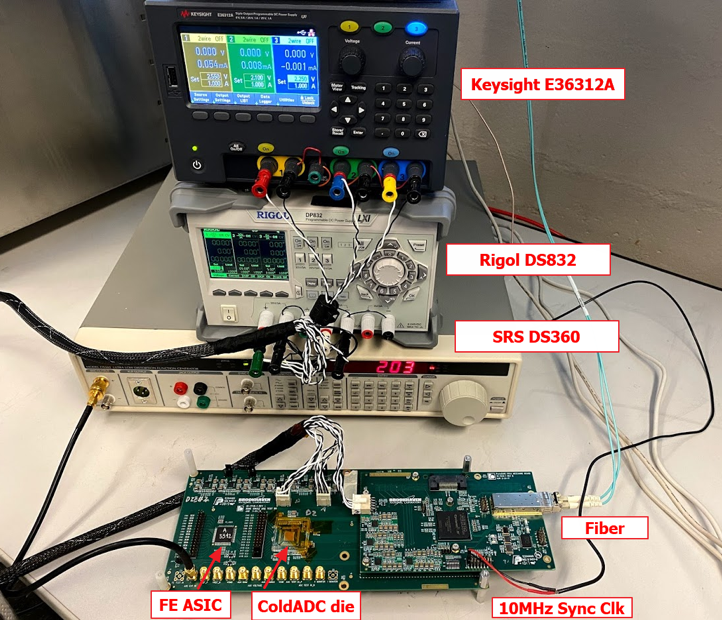
\includegraphics[width=0.85\linewidth]{figures/BNL_testsetup.png}
  \caption{BNL ColdADC (die or chip) test setup.}
  \label{fig:bnl_testsetup}
\end{figure}


Python scripts are implemented to communicate with FPGA mezzanine via UDP protocol and analyze the data collected. A Python-based GUI interface was implemented to display real-time output.

       A similar test setup is built for the QC procedure which is described in Section~\ref{sec:6.1}.

The SFP module on FM cannot work in liquid nitrogen temperature, if cold test is conducted, half of the test board assembly, including FE-ASIC and ColdADC, is submerged in liquid nitrogen. The other half is above liquid nitrogen level, as shown in Figure 5.    
\begin{figure}[!ht]
\centering
 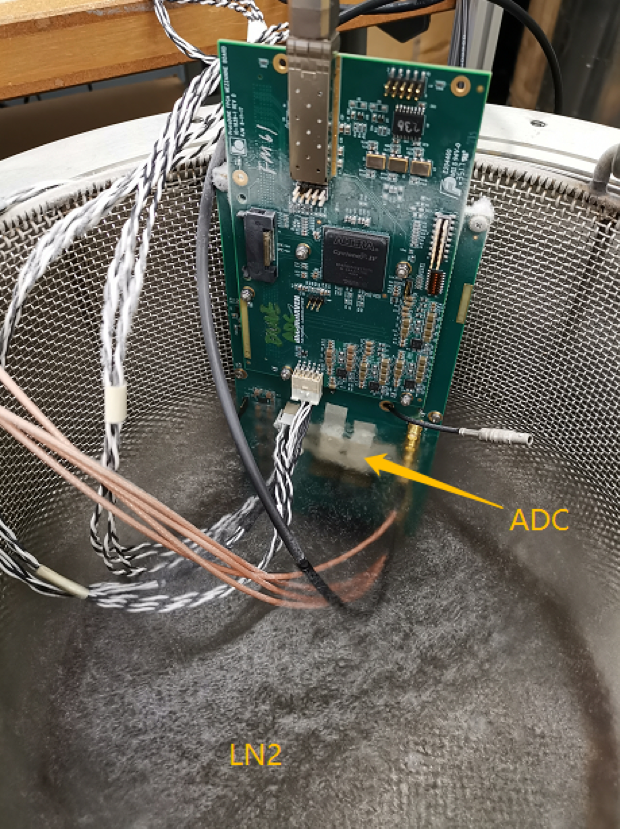
\includegraphics[width=0.85\linewidth]{figures/BNL_coldtest.png}
  \caption{Cold test with ColdADC submerged in LN$_2$.}
  \label{fig:bnl_coldtest}
\end{figure}
